\documentclass[a4paper]{report}
\usepackage[utf8]{inputenc}
\usepackage[T1]{fontenc}
\usepackage[french]{babel}
\usepackage{graphicx}
\usepackage{amsfonts}
\usepackage{float}
\usepackage[export]{adjustbox}

\date{}
\title{Calcul sécurisé, Attaque par faute sur le DES}
\author{Niels Merceron \\ Numéro d'étudiant: 21801038 \\ \\ 
\includegraphics[scale=0.20]{logo-UVSQ-2020-RVB.png}}


\begin{document}
	\maketitle
	
	\newpage
	 \tableofcontents
		\chapter{Attaque par faute sur le DES}
			\section{Description du principe d'attaque par faute}
			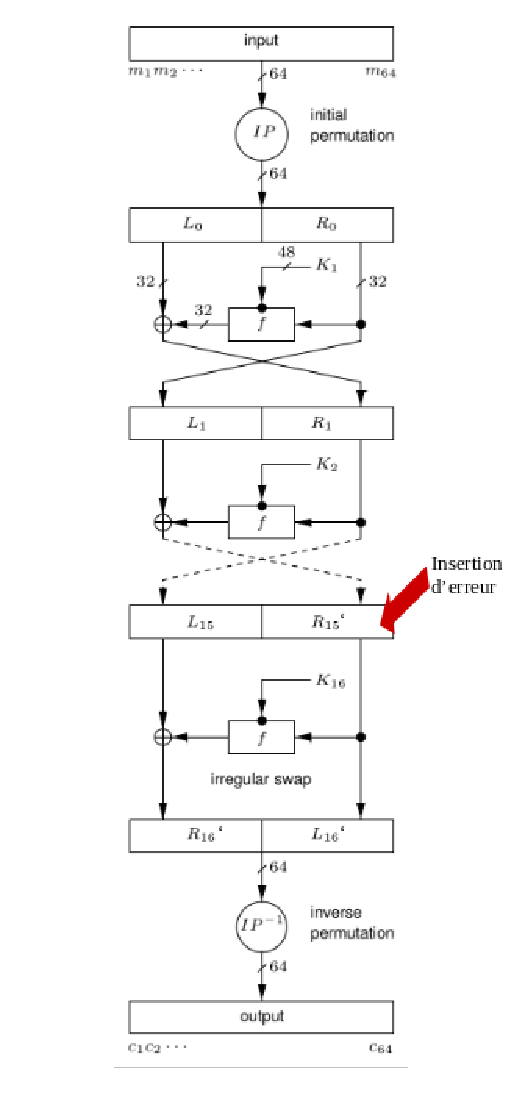
\includegraphics[scale=0.49]{DESFAUTE.pdf} 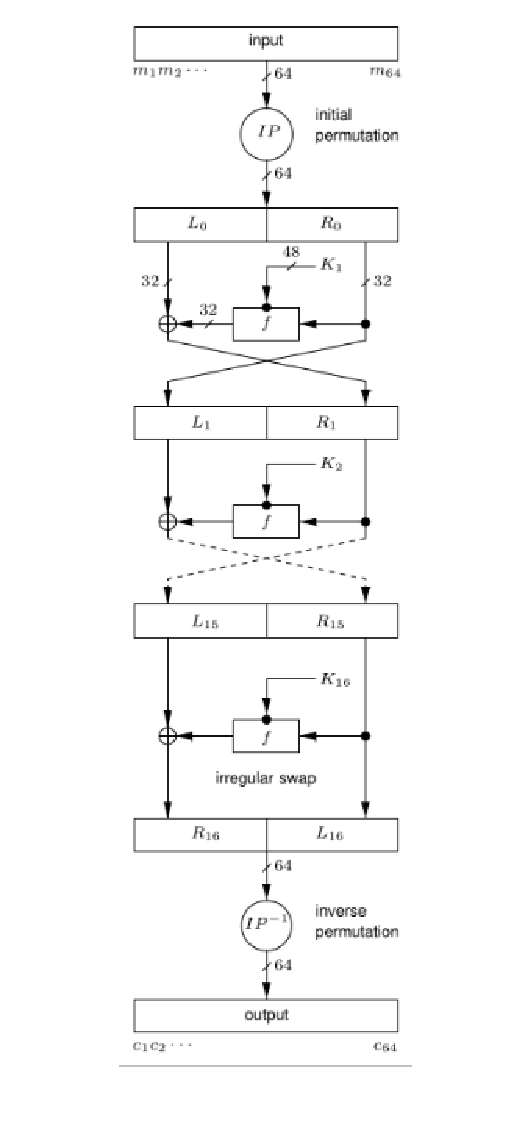
\includegraphics[scale=0.48]{DES.pdf}
			\begin{center}\title{Schéma du DES avec et sans faute}\end{center}
			 
			On va injecté une faute a l'aide d'un laser dans un tour (dans notre cas le 15ème), de cette faute résultera un chiffré différent de celui sans faute.
			De ces Deux chiffrés on les comparera en effectuant divers calcul dessus pour arriver a manipulé quelque chose de simple et qui nous donne de l'information sur la clef secrète.
			Plus précissement, on identifera quel bit est touché par la faute. Une fois le bit identifié on regardera quel fontion sont touchées par ce bit fauté.
			Puis on effectura le calcul des fonctions touchés avec la version non fauté et fauté. Puis on comparera ces deux fonctions pour trouver des informations sur la clef secrète K .
			
			
		\chapter{Application concrète}
			\section{Description de l'attaque par faute}
			Pour commencer on veut obtenir R16 et L16 donc on effectue au chiffré correcte les permutations décrite par IP. On fait la même chose pour obtenir R16' et L16' qui correspondent au chiffré fauté.\\
			On a donc $R16 = R15$ , $L16 = L15\oplus f(R15,K16)$ mais aussi $R16'=R15'$ et $L16'=L15\oplus f(R15',K16)$.
			Pour savoir ou ce situe l'erreur on effectue le calcul suivant $R16\oplus R16' = R15\oplus R15' = R15\oplus R15\oplus \mathcal{E} = \mathcal{E}$. Savoir ou ce situe l'erreur nous aidera plus tard.\\
			
			Une fois cela fait on passe a la partie plus technique.Notre but est de trouver une formule avec ce que nous connaissons, avec K16 dedans et la plus réduite possible.
			On va donc commencer par effectuer :\\
			$L16'\oplus L16 = L15\oplus f(R15',K16) \oplus L15\oplus f(R15,K16) =f(R15',K16)\oplus f(R15,K16)$.\\
			
			une fois cela fait on va écrire explicitement la fonction f. Cette fonction f consiste en une expansion(E) puis on xor le résultat avec $K_i$(dans notre cas $K_{16}$) ensuite le résultat du xor passe dans les Sbox et pour finir passe dans une permutation(P). 
			on obtient donc la formule suivant :
			\begin{center}$L16'\oplus L16 = P(S(E(R_{15}')\oplus K_{16}))\oplus P(S(E(R_{15})\oplus K_{16})) $\end{center}
			
			
			On obtient donc comme partie de clef : B1A6E1869A35
		
		\chapter{Retrouver la clef complète du DES}
			Pour retrouver les 8 bits manquants on peut force brute sur $2^{8}$ valeur et calculer le Des avec chaque clef créé a l'aide des $2^{8}$
			
			On obtient donc comme clef : E65875255B64BA40
		
		\chapter{Fautes sur les tours précédents}
			\section{attaque sur le 14ème tour}
			\section{attaque sur le 13ème tour}
			\section{généralisation sur le nième tour}
		
		\chapter{Contre-mesures}
			\section{Doublé le calcul du DES}
				Une solution assez simple qui nous vient en tête est de calculé deux/plusieurs fois l'algorithme du DES pour le même message puis véfirier si les résultats obtenu a la fin est
				identique.
				Si les résultats sont identique alors il n'y a pas eu d'injection de faute, sinon une faute a été introduite on ne renvoie rien.
				Cependant cette méthode est partiellement efficace car on peut partir du principe que l'attaquant a plusieurs outils similaires pour faire la fautes au même endroit a chaque fois et 
				donc que l'injection de faute soit un succès. 
				Il faudrait donc calculer n+1 fois le DES (n étant le nombre d'outils qu'a l'attaquant) pour espérer s'en protéger ce qui donnerai une compléxité très grande. 
				De plus si on voulais mettre cette solution dans une carte a puce on serait très vite limité au nombre de fois que l'ont puisse calculer le DES.
				La compléxité de cette solution serait de l'ordre K$\times$O(DES), K étant le nombre de fois que l'ont calcul le DES.
			
			\section{rajouté de l'aléatoire/calcul imbriqué}
		
		\chapter{Annexe}


		
\end{document}